\section{Implementierung}


\subsection{Probleme} \label{Probleme}

\begin{enumerate}
    \item Taxi\\
    Für das Taxiproblem \cite{faramaGymnasiumDocumentation} wurde ein 5 x 5 großes Gitternetz implementiert. Der Agent (Taxifahrer) hat dabei die Möglichkeit, sich in alle vier Himmelsrichtungen zu bewegen. Die Aufgabe besteht darin, den Passagier, welcher sich in einer zufälligen Ecke des Gitternetzes befindet, abzuholen und ihn dann zu seinem gewünschten Ziel zu bringen. Dieses ist immer einer der verbleibenden Ecken des Spielfeldes. Um diese Aufgabe noch etwas zu erschweren, wurden zusätzlich noch Wände in das Gitternetz integriert. Diese befinden sich an den gleichen Positionen und verhindern Bewegungen in bestimmte Richtungen.

    Für das Bewältigen dieser Aufgabe kann der Agent zu jedem Zeitpunkt zwischen sechs Actions entscheiden; Bewegung in jeweils einer der vier Himmelsrichtungen, Aufnehmen des Passagiers und das Absetzen des Passagiers. Natürlich sind nicht alle Actions zu jedem Zeitpunkt sinnvoll. 

    Der Zustand des Gitternetzes kann durch 500 diskrete States beschrieben werden. Diese Anzahl ergibt sich aus der Multiplikation der 25 möglichen Position des Taxis, der fünf möglichen Positionen des Passagiers (beinhaltet den Fall, dass sich der Passagier im Taxi befindet), mit den vier möglichen Zielorten.

    Da das Abliefern des Passagiers auf dem richtigen Feld das Ziel der Aufgabe ist, bekommt der Agent dafür auch die höchste Belohnung. Damit die Erfüllung der Aufgabe so effizient wie möglich durchgeführt wird, bekommt der Agent für jede Action, die er durchführt und die nicht zu einer Belohnung führt, eine kleine Strafe. Zudem wird der Agent stark bestraft, wenn er den Passagier an einem falschen Ort absetzt oder versucht, einen Passagier an einer falschen Position aufzunehmen.
    \begin{figure}[H]
        \centering
        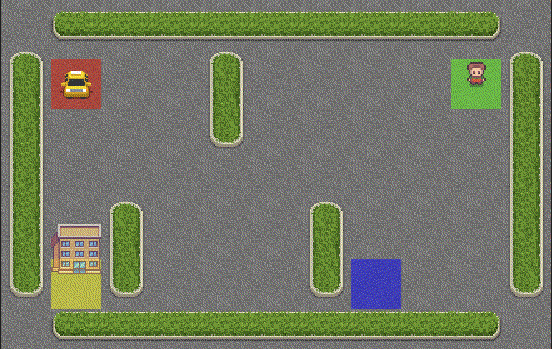
\includegraphics[scale=0.7]{taxi}
        \caption{Taxi Environment}
        \label{fig:taxi_env}
    \end{figure}
    
    \newpage
    
    \item Cliff\\
    Wie für das Taxiproblem wurde auch für das Cliff Problem \cite{faramaGymnasiumDocumentation} ein Gitternetz implementiert. Dieses besitzt eine Größe von 4 x 12. Die Aufgabe des Agent besteht darin, von einer Seite des Gitternetzes zur anderen zu gelangen, ohne dabei in die auf dem Feld befindliche Klippe zu fallen. Als Klippe wurden alle Felder definiert, welche sich auf dem direkten Weg zwischen Agent und Ziel befinden. Der Agent hat somit die Aufgabe, um diese Klippe herum zu navigieren und so das Ziel zu erreichen. Um die Herangehensweise der verschiedenen Algorithmen besser vergleichen zu können, befinden sich bei diesem Experiment alle Objekte (Agent, Klippe, Zielpunkt) zu Beginn jeder Episode an derselben Position.

    Damit sich der Agent auf dem Feld bewegen kann, stehen ihm vier verschiedene Actions zur Verfügung, welche den Agent jeweils um ein Feld in einer der Himmelsrichtungen verschiebt.

    Um den Zustand des Environments zu beschreiben, ist die aktuelle Position des Agent ausreichend. Insgesamt gibt es 48 (4 × 12) verschiedene Positionen auf dem Feld. Da das Betreten der Klippenfelder jedoch zum Ende der Episode führt, sind diese Positionen kein gültiger State. Gleiches gilt auch für die Zielposition. Bei zehn Klippen und einem Ziel ergeben sich so 37 States.

    Neben dem Erreichen des Ziels ist es besonders wichtig, dass der Agent nicht in die Klippe fällt. Daher ist dies mit einer hohen Bestrafung für den Agent versehen. Zudem soll das Ziel so schnell wie möglich erreicht werden. Aus diesem Grund ist, wie auch bei dem Taxi Problem, jede Action mit einer kleinen Strafe belegt. Eine explizite Belohnung des Agent ist für diesen Anwendungsfall nicht nötig, da das Ziel zum Ende der Episode führt und das beste Ergebnis somit jenes ist, welches zur geringsten Bestrafung führt.

    \begin{figure}[H]
        \centering
        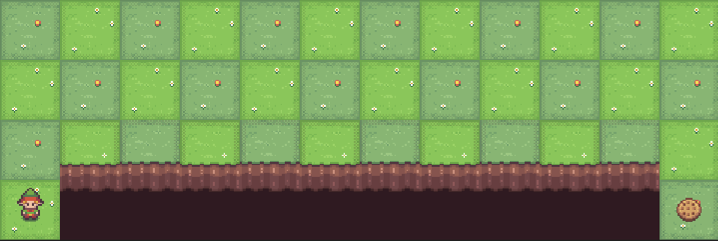
\includegraphics[scale=0.7]{cliff}
        \caption{Cliff Environment}
        \label{fig:cliff_env}
    \end{figure}
    
    \item Frozen Lake\\
    Auch das Frozen Lake Problem \cite{faramaGymnasiumDocumentation} ist auf einem Gitternetz aus Feldern implementiert. Einige Felder sind Eisplatten, die der Agent sicher betreten kann, während andere Felder Löcher darstellen, in die der Agent fallen kann und damit das Spiel verliert. Das Ziel des Agent besteht darin, sicher zum Ziel zu gelangen, welches sich auf der anderen Seite des Sees (Gitternetz) befindet. Die besondere Herausforderung bei diesem Problem sind die Eisplatten. Bewegt sich der Agent auf einer dieser Platten in eine bestimmte Richtung besteht eine Chance, dass er ausrutscht und sich in eine andere Richtung bewegt.

    Wie auch beim Cliff Problem kann der Agent nur durch Bewegung mit dem Environment interagieren und hat somit vier Actions zur Verfügung.


    Ein 4 x 4 großes Environment mit vier Löchern hat somit 11 mögliche States (16 Felder minus die Löcher und des Ziels) 

    Die Struktur des Rewards ist für dieses Problem simpel. Der Agent wird belohnt, wenn er das Ziel erreicht und das Spiel wird beendet, wenn er in ein Loch fällt.
    
    \begin{figure}[H]
        \centering
        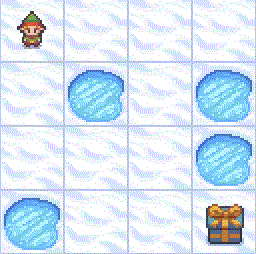
\includegraphics[scale=0.7]{frozen_lake}
        \caption{Frozen Lake Environment}
        \label{fig:frozen_env}
    \end{figure}


\end{enumerate}

\subsection{Optimierung der Hyperparameter}
Die theoretischen Grundlagen der Hyperparameter wurden bereits in \ref*{Def_Hyperparameter} \nameref{Def_Hyperparameter} erläutert. Um konkrete Werte für die im Rahmen dieser Arbeit untersuchten Probleme zu finden, wurden einige Versuche durchgeführt. 
Als Ausgangslage wurde die in Tabelle \ref{tab:hyperBasic} dargestellten Werte angenommen. Im Folgenden werden diese initialen Werte anhand von Experimenten für die verschiedenen Algorithmen und Probleme optimiert.

\begin{table}[h]
    \caption{Hyperparameter Ausgangslage}
    \label{tab:hyperBasic}
    \centering
    \rowcolors{2}{white}{lightgray} 
    \begin{tabular}{>{\itshape}0l0l}\hline % used >{\itshape} in order to be able to remove the repeated occurences of \textit in the first column, used l type columns instead of c columns for a cleaner look, added small vertical space above and below the rows with the help of the cellspace package, removed all vertical lines
    \textup{Paramater}          & Wert\\\hline
    num\_episodes               & 1000\\
    max\_steps\_per\_episode    & 1000\\
    learning\_rate              & 0.1\\
    discount\_rate              & 0.99\\
    exploration\_rate           & 1\\
    max\_exploration\_rate      & 1\\
    min\_exploration\_rate      & 0.01\\
    exploration\_decay\_rate    & 0.005\\\hline
    \end{tabular}
\end{table}

\begin{itemize}
    \item Anzahl an Episoden\\
    Als optimale Anzahl an Episoden wird der Punkt gewählt, ab wann sich der Agent nicht mehr verbessert. So wird ein zu langes Training vermieden. 
    Dieser Punkt lässt sich sehr gut in einer grafischen Darstellung der erreichten Belohnung des Agent im Vergleich zu den während des Trainings durchlaufenen Episoden ablesen. 
    Die Rohdaten aus dem Training sind aufgrund der Exploration sehr verrauscht und der eigentliche Trainingsfortschritt ist nur schwer zu erkennen.
    Um die Grafik lesbarer zu machen wurde ein gleitender Durchschnitt auf die Daten angewandt. Der Effekt dieser Operation wurde in der Abbildung \ref{fig:NumOfEpisods_MovingAVG} veranschaulicht.

    \begin{figure}[H]
        \centering
        \begin{subfigure}{.5\textwidth}
          \centering
          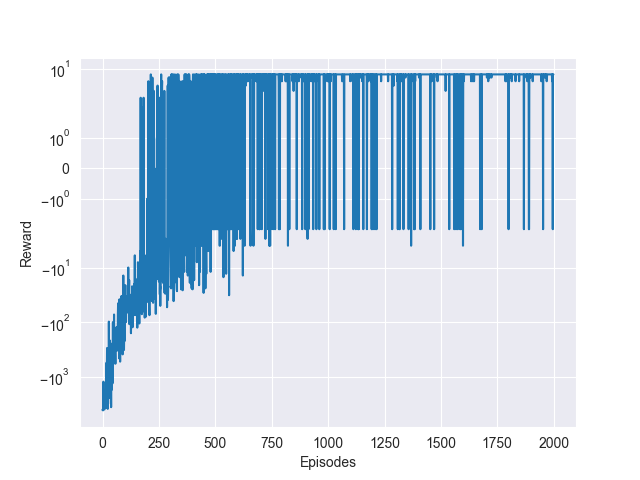
\includegraphics[width=1\linewidth]{Hyper_Data_Raw}
          \caption{Rohdaten}
          \label{fig:NumOfEpisods_Raw}
        \end{subfigure}%
        \begin{subfigure}{.5\textwidth}
          \centering
          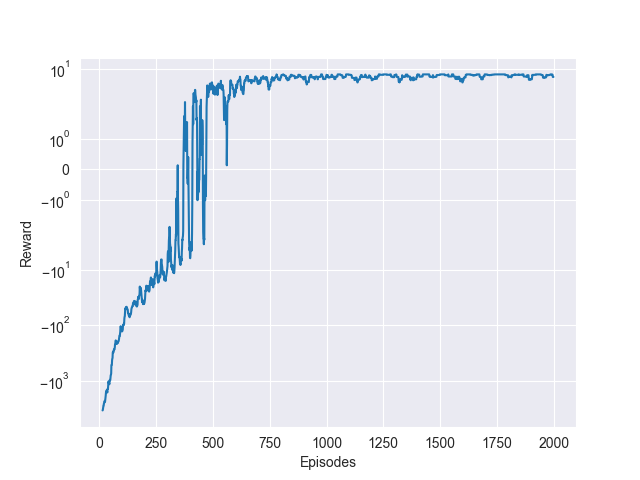
\includegraphics[width=1\linewidth]{Hyper_Data_Clean}
          \caption{Gleitender Durchschnitt}
          \label{fig:NumOfEpisods_clean}
        \end{subfigure}
        \caption{Anwendung gleitender Durchschnitt}
        \label{fig:NumOfEpisods_MovingAVG}
    \end{figure}

    \item Maximale Anzahl an Steps pro Episode\\
    Für die Festlegung dieses Hyperparameters wurde zunächst der Trainingsverlauf des initialen Wertes mit dem Trainingsverlauf von deutlich erhöhten und reduzierten Werten verglichen.
    So wurde der Einfluss des Parameters analysiert und eine erste Tendenz festgestellt.
    Darauf wurde weitere Vergleiche durchgeführt, um den optimalen Wert zu bestimmen.

    \item Learning Rate\\
    Wie auch bei der Festlegung der maximalen Anzahl an Steps pro Episode wurde auch für die Learning Rate der initiale Wert verändert und die Auswirkungen anhand von Graphen analysiert.

    \item Discount Rate\\
    Die Discount Rate wurde ebenfalls ermittelt, indem die Auswirkungen einer Veränderung des Hyperparameters untersucht wurden. 
    Der initial gewählte Wert für die Discount Rate ist sehr nah am Maximum des möglichen Wertebereichs. 
    Dementsprechend wurde ausschließlich eine Reduzierung des Parameters untersucht.

    \item Exploration Rate\\
    Damit sich der Wert der Exploration Rate über den Verlauf des Trainings verändert, sind insgesamt vier Parameter implementiert. 
    Die Obergrenze für den Wert, sowie der Startwert, sind initial auf Eins festgelegt. 
    Zu Beginn hat der Agent noch kein Wissen über das Environment, eine Exploitation ist somit nicht sinnvoll. 
    Eine Reduzierung des Wertes führt somit nur zu einem langsamen Trainingsverlauf. 
    Die Abnahmerate und der minimale Wert sind durch Experimente, wie die vorherigen drei Hyperparameter, ermittelt worden.
\end{itemize}


\subsection{Vergleichen von Algorithmen}

Nach dem im vorangegangen Kapitel die Implementation des Vergleichens der Hyperparameter beschrieben wurde, befasst sich dieser Abschnitt mit dem Verlgeichen der beiden Algorithmen Q-Learning und SARSA. 
Um den bestmöglichen Vergleich zu gewährleisten wurden geeignete Parameter für beide Algorithmen und die jeweiligen Probleme gewählt. Diese Parameter sind den Tabellen \ref{tab:Taxi} bis \ref{tab:FrozenLake} aufgeführt. Bei der Analyse wurden alle drei Probleme, welche in \ref{Probleme} bereits erläutert wurden, berücksichtigt.



   
\begin{table}[!htb]
    % \caption{Global caption}
    \begin{minipage}{.5\linewidth}
        \caption{Taxi Paramater}
        \label{tab:Taxi}
        \centering
        \rowcolors{2}{white}{lightgray} 
        \begin{tabular}{>{\itshape}0l0l0l}\hline % used >{\itshape} in order to be able to remove the repeated occurences of \textit in the first column, used l type columns instead of c columns for a cleaner look, added small vertical space above and below the rows with the help of the cellspace package, removed all vertical lines
        \textup{Paramater}          & Q-Learning    & SARSA\\\hline
        num\_episodes               & 3000          & 3000\\
        max\_steps\_per\_episode    & 2000          & 2000\\
        learning\_rate              & 0.4           & 0.1\\
        discount\_rate              & 0.6           & 0.99\\
        exploration\_rate           & 1          & 1\\
        max\_exploration\_rate      & 1          & 1\\
        min\_exploration\_rate      & 0.01          & 0.01\\
        exploration\_decay\_rate    & 0.01          & 0.1\\\hline
        \end{tabular}
    \end{minipage}%
    \begin{minipage}{.5\linewidth}
        \caption{Cliff Paramater}
        \label{tab:Cliff}
        \centering
        \rowcolors{2}{white}{lightgray} 
        \begin{tabular}{>{\itshape}0l0l0l}\hline % used >{\itshape} in order to be able to remove the repeated occurences of \textit in the first column, used l type columns instead of c columns for a cleaner look, added small vertical space above and below the rows with the help of the cellspace package, removed all vertical lines
        \textup{Paramater}          & Q-Learning    & SARSA\\\hline
        num\_episodes               & 1500          & 1500\\
        max\_steps\_per\_episode    & 750           & 1000\\
        learning\_rate              & 0.4           & 0.05\\
        discount\_rate              & 0.1           & 0.99\\
        exploration\_rate           & 1          & 1\\
        max\_exploration\_rate      & 1          & 1\\
        min\_exploration\_rate      & 0.01          & 0.01\\
        exploration\_decay\_rate    & 0.01          & 0.1\\\hline
        \end{tabular}
    \end{minipage} 
\end{table}

\begin{table}[h]
    \caption{Frozen Lake Paramater}
    \label{tab:FrozenLake}
    \centering
    \rowcolors{2}{white}{lightgray} 
    \begin{tabular}{>{\itshape}0l0l0l}\hline % used >{\itshape} in order to be able to remove the repeated occurences of \textit in the first column, used l type columns instead of c columns for a cleaner look, added small vertical space above and below the rows with the help of the cellspace package, removed all vertical lines
    \textup{Paramater}          & Q-Learning    & SARSA\\\hline
    num\_episodes               & 2000          & 2000\\
    max\_steps\_per\_episode    & 500           & 2000\\
    learning\_rate              & 0.4           & 0.3\\
    discount\_rate              & 0.2           & 0.99\\
    exploration\_rate           & 1          & 1\\
    max\_exploration\_rate      & 1          & 1\\
    min\_exploration\_rate      & 0.01          & 0.01\\
    exploration\_decay\_rate    & 0.005          & 0.1\\\hline
    \end{tabular}
\end{table}


Zum Vergleich der Algorithmen wurden die Rewards und Steps während des Trainings aufgenommen und anschließend in Plots anschaulich dargestellt. 
Dabei wurde je nach Problem eine logarithmische Skalar auf der y-Achse genutzt, um die Daten anschaulicher zu gestalten. Zusätzlich wird ein Rolling Window Ansatz gewählt, sodass immer 15 Werte zusammengefasst werden. Dies sorgt dafür das einzelne Peaks zwar weniger auffallen, dafür der Gesamttrend im Verlauf der Trainingsepisoden aber besser zu erkennen ist.


    
